\documentclass[12pt]{article}
\usepackage{amsmath}
\usepackage{amssymb}
\usepackage{multirow}
\usepackage{fullpage}
\usepackage{graphicx}
\usepackage{amsthm}
\usepackage{imakeidx}
\makeindex
\title{Quick Sort Partitioning Algorithm}
\author{Shubham Sharma}
\date{\today}
\begin{document}
\maketitle
\tableofcontents
\listoftables
\listoffigures
\newpage
\section{Introduction}
\begin{figure*}[h]
        \begin{center}
                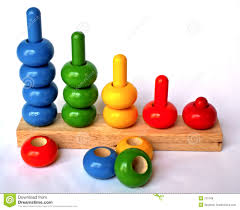
\includegraphics[width=0.7\columnwidth]{index1}
        \end{center}
        \caption{Sorting}
        \label{fig:shapes}
\end{figure*}
 
\par Sorting is nothing but storage of data in \index{sorted order}, it can be in ascending or descending order. The term Sorting comes into picture with the term Searching. There are so many things in our real life that we need to search, like a particular record in database, roll numbers in merit list, a particular telephone number, any particular page in a book etc. Sorting arranges data in a sequence which makes searching easier. Every record which is going to be sorted will contain one key. Based on the key the record will be sorted.
\par There are many techniques for sorting. Implementation of particular sorting \index{technique} depends upon situation. \index{Sorting} techniques mainly depends on two parameters. First parameter is the execution time of program, which means time taken for execution of program. Second is the space, which means space taken by the program\cite{Wiki}.
\newpage
\section{Quick Sort}
\subsection{Algorithm}
\par Quick Sort is a \index{Divide and Conquer} algorithm. It picks an element as \index{pivot} and partitions the given array around the picked pivot. There are many different versions of quickSort that pick pivot in different ways.
\begin{itemize}
\item Always pick first element as pivot.
\item Always pick last element as pivot.
\item Pick a random element as pivot.
\item Pick median as pivot.
\end{itemize}
\par The key process in quickSort is \index{partition}(). Target of \index{partitions} is, given an array and an element x of array as pivot, put x at its correct position in sorted array and put all smaller elements (smaller than x) before x, and put all greater elements (greater than x) after x. All this should be done in linear time\cite{Mcgraw}.
\subsection{Partition Algorithm}
\par To complete the \index{implementation}, we need to implement the \index{partitioning} method. We use the following general strategy: First, we arbitrarily choose a[lo] to be the partitioning item—the one that will go into its final position. Next, we scan from the left end of the array until we find anentry that is greater than (or equal to) the partitioning item, and we scan from the right end of the array until we find an entry less than (or equal to) the partitioning item.\cite{Knuth}
\begin{figure*}[h]
        \begin{center}
                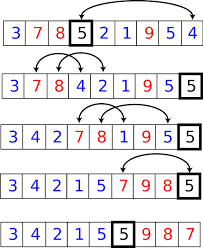
\includegraphics[scale=0.7]{index}
        \end{center}
        \caption{Partitioning}
        \label{fig:shapes}
\end{figure*}
 
\par Items that stopped the scans are out of place in the final \index{partitioned array}, so we exchange them. When the scan indices cross, all that we needto do to complete the partitioning process is to exchange the partitioning item a[lo] with the rightmost entry of the left subarray (a[k]) and return its index k. 
\subsection{Pseudocode}
\begin{figure*}[h]
        \begin{center}
                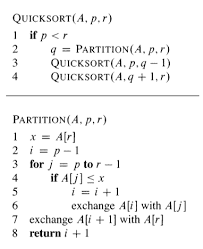
\includegraphics[scale=0.7]{index5}
        \end{center}
        \caption{Pseudocode}
        \label{fig:shapes}
\end{figure*}
\subsection{Analysis of Quicksort}
\subsubsection{Time Complexity}
\par Time taken by QuickSort in general can be written as following\cite{Hoare}.
\begin{equation}
T(n) = T(k) + T(n-k-1) + \theta(n)
\end{equation}
\par The first two terms are for two recursive calls, the last term is for the partition process. k is the number of elements which are smaller than pivot.\\
The time taken by QuickSort depends upon the input array and partition strategy. Following are three cases.\\
\par \textbf {Worst Case:}The worst case occurs when the partition process always picks greatest or smallest element as pivot. If we consider above partition strategy where last element is always picked as pivot, the worst case would occur when the array is already sorted in increasing or decreasing order. Following is recurrence for worst case\cite{Hoare}.
\begin{equation}
T(n) = T(n-1) + \theta(n)
\end{equation}
\par The solution of above recurrence is O($n^2$).\\ 
\par {\bfseries{Best Case:}}
The best case occurs when the partition process always picks the middle element as pivot. Following is recurrence for best case\cite{Hoare}.
\begin{equation}
T(n) = 2T(n/2) + \theta(n)
\end{equation}
\par The solution of above recurrence is O(nLog(n)) 
\cite{master}\\
\par {\textbf {Average Case :}}To do average case analysis, we need to consider all possible permutation of array and calculate time taken by every permutation. Following is the Time complexity \cite{cormen}
\begin{equation}
T(n)=2nlog(n) - 2.84n + O(1)
\end{equation}
\par Solution of above recurrence is also O(nLogn) \cite{cormen}
\subsubsection{Auxiliary Space}
\hspace{10pt} \textit O(log n) extra space for recurrence 
\section{Selection Sort}
\subsection{Algorithm}
\par The selection sort algorithm sorts an array by repeatedly finding the minimum element (considering ascending order) from unsorted part and putting it at the beginning. The algorithm maintains two subarrays in a given array.
\begin{enumerate}
\item The subarray which is already sorted.
\item Remaining subarray which is unsorted.
\end{enumerate}
\par In every iteration of selection sort, the minimum element (considering ascending order) from the unsorted subarray is picked and moved to the sorted subarray. 
\newpage
\subsection{Pseudocode}
\begin{figure*}[h]
        \begin{center}
                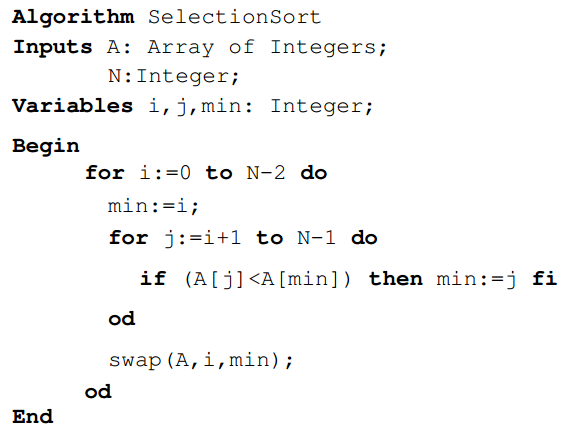
\includegraphics[scale=0.7]{Untitled}
        \end{center}
        \caption{Pseudocode}
        \label{fig:shapes}
\end{figure*}
\vspace{10pt}
\subsection{Analysis of Selection Sort}
\subsubsection{Time Complexity}
\par O($n^2$) as there are two nested loops.
\subsubsection{Auxiliary Space}
\textit O(1)
\newpage
\section{Comparison Between Quicksort and Selection Sort}
\subsection{Time Complexity}
\vspace{-5pt}
\begin{table}[h]
    \centering
    \begin{tabular}{|c|c|c|}
         \hline
Cases & Selection Sort & Quick Sort \\
\hline
Worst Case & \textit{O($n^2$)} & \textit{O($n^2$)}\\
\hline
Best Case & \textit{O($n^2$)} & \textit{O(nlog(n))}\\
\hline
Average Case & \textit{O($n^2$)} & \textit{O(nlog(n))}\\
\hline
    \end{tabular}
    \caption{Time Complexity Analysis}
    \label{tab:my_label}
\end{table}
\vspace{-10pt}
\subsection{Auxiliary Space}
\begin{table}[h]
    \centering
   \begin{tabular}{|c|c|}
\hline
Selection Sort & Quick Sort \\
\hline 
\textit{O(1)} & \textit{O(log(n))}\\
\hline
\end{tabular}
    \caption{Space Complexity Analysis}
    \label{tab:my_label}
\end{table}
\begin{figure*}[h]
        \begin{center}
                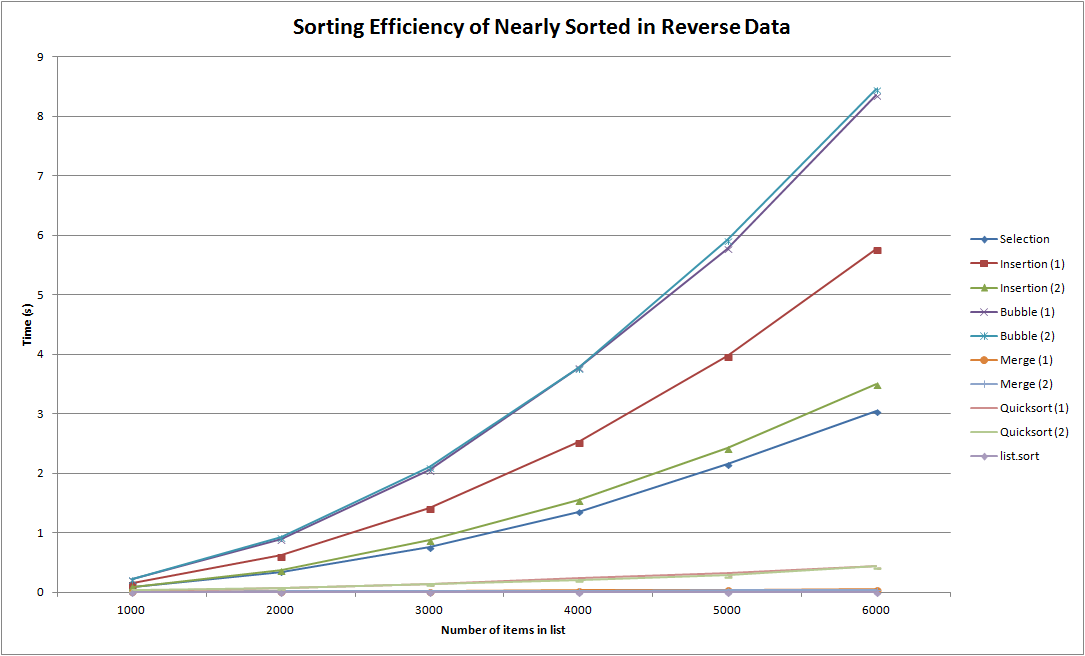
\includegraphics[scale=0.5]{graph3}
        \end{center}
        \caption{Analysis of Different Sorting Algorithms}
        \label{fig:shapes}
\end{figure*}
\newpage
\begin{figure*}[h]
        \begin{center}
                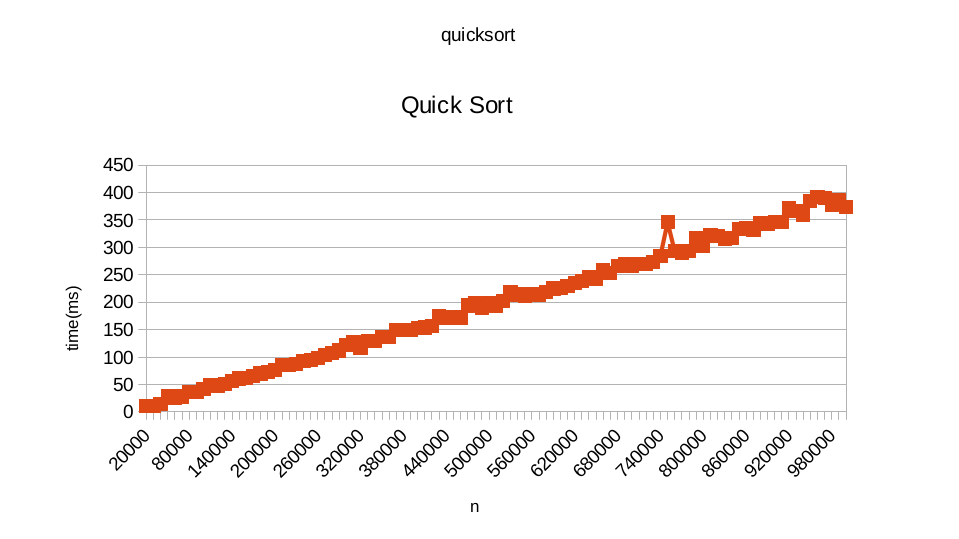
\includegraphics[scale=0.5]{XxdQf}
        \end{center}
        \caption{Performance}
        \label{fig:shapes}
\end{figure*}
\par 
Quicksort is a well-known sorting algorithm  that, on average, makes O(n log n) comparisons to sort n items. However, in the worst case, it makes O(n2) comparisons. Typically, quicksort is significantly faster than other O(n log n) algorithms, because its inner loop can be efficiently implemented on most architectures, and in most real-world data, it is possible to make design choices which minimize the probability of requiring quadratic time. Through the analysis of Time and Space Complexity between Quick Sort and Selection Sort it can be concluded that Quick Sort is generally more efficient that Selection Sort.
\par  Advantages of Quick Sort  include the efficient average case compared to any aforementioned sort algorithm, as well as the elegant recusrive definition, and the popularity due to its high efficiency. Disadvantages include the difficulty of implementing the partitioning algorithm and the average efficiency for the worst case scenario, which is not offset by the difficult implementation. 
 \newpage
\medskip
\bibliographystyle{unsrt}
\bibliography{example1}
\bibliographystyle{alpha}
\printindex
\end{document}
